\documentclass{beamer}
\usetheme{CambridgeUS} % replace it with Boadilla if you want no section bar
%\usecolortheme{crane} % other ones: dove, dolphin, rose, seahorse, orchid, crane, seagull, lily, wolverine
%\usefonttheme{serif} 
\usefonttheme[onlymath]{serif} % uncomment if you want it just for math

\setbeamertemplate{navigation symbols}{}  % comment to have nagivation

\usepackage[compress,comma,authoryear]{natbib}
\usepackage{tikz}
\usetikzlibrary{mindmap,trees}
\usepackage{amsmath,mathtools}
\usepackage{amsthm}
\usepackage{booktabs}
\usepackage{graphicx,epstopdf}
\usepackage{hyperref}


\definecolor{blue}{RGB}{0,114,178}
\definecolor{orange}{RGB}{213,94,0}
\definecolor{red}{RGB}{190,0,0}
\definecolor{yellow}{RGB}{240,228,66}
\definecolor{green}{RGB}{0,158,115}
\definecolor{Lblue}{RGB}{0,197,155}
\definecolor{Dblue}{RGB}{0,76,119}
\definecolor{Lgreen}{RGB}{180,255,230}

\hypersetup{
	colorlinks=false,
	linkbordercolor = {white},
	linkcolor = {blue}
}
\definecolor{MyBackground}{RGB}{245,245,245}

\setbeamercolor{frametitle}{fg=blue}
\setbeamercolor{title}{fg=blue}
\setbeamertemplate{footline}[frame number]
\setbeamertemplate{navigation symbols}{} 
\setbeamertemplate{itemize item}[circle]%{$\bigstar$}
\setbeamertemplate{itemize subitem}{$\bigstar$}
\setbeamercolor{itemize item}{fg=blue}
\setbeamercolor{itemize subitem}{fg=blue}
\setbeamercolor{enumerate item}{fg=blue}
\setbeamercolor{enumerate subitem}{fg=blue}
\setbeamercolor{button}{bg=MyBackground,fg=blue}
\setbeamercolor*{palette primary}{use=structure,fg=blue,bg=white}
\setbeamercolor*{palette secondary}{use=structure,fg=white,bg=Dblue}
\setbeamercolor*{palette tertiary}{use=structure,fg=white,bg=blue}
\setbeamercolor*{palette quaternary}{fg=white,bg=black}
\setbeamercolor*{palettes quaternary}{fg=white,bg=Lgreen}
%\setbeamercolor{titlelike}{parent=structure,bg=Lgreen}
%\setbeamercolor{title in head/foot}{bg=Lgreen,fg=orange}

\setbeamertemplate{enumerate item}{%
	\usebeamercolor[bg]{item projected}%
	\raisebox{1.5pt}{\colorbox{blue}{\color{fg}\footnotesize\insertenumlabel}}%
}





\begin{document}
	\title[Econometrics 2]{Econometrics 2 (M.Sc.)}
	\subtitle{Selection Bias and Experiments}
	\author[Mohammad Hoseini]{Mohammad Hoseini}
	
	%\institute[IMPS]{Institute for Management and Planning Studies (IMPS)}
	
	\date[Spring 2024]{Spring 2024 \\
	\vspace{10pt} @metrics2
}
	
\begin{frame}[plain]
	\titlepage
\end{frame}


\section{Selection bias \& experiments}



\subsection{The selection problem}

\begin{frame}{Regression doesn't necessarily mean causality}
In the previous lectures, we discussed dealing with the standard error issues, linear vs. discrete outcome models, etc.\bigskip

All of them do not necessarily imply that a regression coefficient can be given a causal interpretation.\bigskip

Remember the definition of causality in potential outcome model: 
Potential outcome corresponding to the treatment on/off.\medskip

It relies on ``counter-factual'' to make a causal statement.\medskip

\end{frame}

\begin{frame}{Examples of outcome and treatment (intervention)}
\begin{center}
\begin{tabular}{l|l}
	Treatment ($D$) & Outcome ($y$) \\
	\hline
	
	exercise & blood pressure\\
	drug & Cholesterol\\
	going to hospital & health \\
	going to school & income as an adult  \\
	job training program & employment  \\
	size of the class & educational quality \\
	getting a loan & production  \\
	$\qquad\vdots$ &	$\qquad\vdots$ \\
\end{tabular}
\end{center}

\end{frame}

\begin{frame}{The potential outcome}
Consider a binary treatment taking on 0 or 1.\bigskip

$Y_i^D , D=0,1$ is the potential outcome when individual or unit $i$ receives treatment $D$ \textbf{\color{red}exogenously}.
\begin{itemize}
\item $Y_i^0$ is the potential outcome if $i$ doesn't receive treatment $D_i=0$.
\item $Y_i^1$ is the potential outcome if $i$ receives treatment $D_i=1$.
\end{itemize}\bigskip

Example:\begin{itemize}
\item $Y_i^0$: blood pressure with exercise ``forced out''
\item $Y_i^1$: blood pressure with exercise ``forced in''

\end{itemize}

``forced in'' and ``forced out'' reflect the notion of intervention.\medskip

In other words, the subjects do not ``self-select'' for the treatment.


\end{frame}

\begin{frame}{The treatment effect}
The simplest and most common way of measuring treatment effect \pause is average difference in potential outcomes:
\[E[Y_i^1-Y_i^0]=E[Y_i^1]-E[Y_i^0]\]\pause
Some other alternatives:
\begin{itemize}
\item Median or $\alpha$ quantile: $Q_\alpha(Y_i^1-Y_i^0)$
\item Proportional effect: $E[Y_i^1-Y_i^0]/E[Y_i^0]=E[Y_i^1]/E[Y_i^0]-1$
\item But only $E[Y_i^1-Y_i^0]$ can be linearly separated.
\end{itemize}\bigskip

Note that ``no treatment effect'' means $E[Y_i^1]=E[Y_i^0]$ not $Y_i^1=Y_i^0$.

\end{frame}

\begin{frame}{Observed outcome}
The $Y_i$ we observe in practice is the actual (not potential) outcome:
\[Y_i=\begin{cases} 
Y_i^0\text{ if }D_i=0\\
Y_i^1\text{ if }D_i=1
\end{cases} \text{ or } \quad Y_i=Y_i^0+(Y_i^1-Y_i^0)D_i \]\pause
We do not observe $Y_i^1$ if $D_i=0$ and $Y_i^0$ if $D_i=1$.\bigskip\pause

Thus, the mean difference between treated and not treated groups in the observed data is
\[ E[Y_i^1|D_i=1]-E[Y_i^0|D_i=0] \]
This is not necessarily equal to $E[Y_i^1-Y_i^0]$

\end{frame}

\begin{frame}{Example: effect of going to hospital on health}
$D=0/1$ is not going / going to hospital and $Y$ is health status.
\begin{itemize}
\item For healthy people: $\quad Y_i^0=10,\quad Y_i^1=8$
\item For sick people: $\qquad Y_i^0=2, \quad Y_i^1=6$
\end{itemize}\medskip
Under self-selection, assume only sick people go to hospital. Then
\begin{itemize}
\item The observed effect: $E[Y_i^1|D_i=1]-E[Y_i^0|D_i=0]=6-10=-4$
\item Going to hospital reduces health status by -4?!
\end{itemize}\bigskip

If unobservable counter-factuals $Y_i^1|D_i=0$ and $Y_i^0|D_i=1$ are known
\begin{itemize}
\item The treatment effect for sick people is $E[Y_i^1-Y_i^0|D_i=1]=6-2=+4$, but without hospital their health status is 8 unit less than healthy
\item Assume one half of the population is sick and one half is healthy,
treatment effect for all people $E[Y_i^1-Y_i^0]=0.5(8+6-10-2)=1$.

\end{itemize}

\end{frame}

\begin{frame}{The selection bias}
%\[E[Y_i^1-Y_i^0]= E[Y_i^1|D_i=1]{\color{blue}+E[Y_i^1|D_i=0]-E[Y_i^0|D_i=1]}-E[Y_i^0|D_i=0] \]\medskip\pause
Observed effect: $E[Y^1_{i}|D_i=1]-E[Y^0_{i}|D_i=0]$
%\[=E[Y^1_{i}|D_i=1]-E[Y^0_{i}|D_i=1]+E[Y^0_{i}|D_i=1]-E[Y^0_{i}|D_i=0] \]
\[=\underbrace{E[Y^1_{i}-Y^0_{i}|D_i=1]}_{\text{Treatment effect on the treated}}+\underbrace{E[Y^0_{i}|D_i=1]-E[Y^0_{i}|D_i=0]}_{\text{Selection bias 1}} \]\[=\underbrace{E[Y^1_{i}-Y^0_{i}|D_i=0]}_{\text{Treatment effect on the not treated}}+\underbrace{E[Y^1_{i}|D_i=1]-E[Y^1_{i}|D_i=0]}_{\text{Selection bias 2}} \]\medskip\pause

Assume $w_0$ and $w_1$ are the shares of not treated ($D_i=0$) and treated ($D_i=1$) in population:
\[\text{Observed effect:  } E[Y^1_{i}|D_i=1]-E[Y^0_{i}|D_i=0]=\underbrace{E[Y^1_{i}-Y^0_{i}]}_{\text{Treatment effect}}\] \[+\underbrace{w_1\big(E[Y^0_{i}|D_i=1]-E[Y^0_{i}|D_i=0]\big)+w_0\big(E[Y_i^1|D_i=1]-E[Y_i^1|D_i=0]\big)}_{\text{Selection bias}} \]
Selection bias is caused by the difference between potential outcomes of treatment and control groups with or without treatment.
\end{frame}

\begin{frame}{The selection bias problems}


The selection bias can be so large that it completely masks the treatment effect (like the previous example)\bigskip

The selection bias can have the same or opposite sign as the treatment effect and thus exaggerate or understate the true effect.
\begin{itemize}
\item going to college on wage (+) 
\item going to hospital on health (--)
\end{itemize}\bigskip

When the treatment and control groups are the same the selection bias vanishes.
\end{frame}

\begin{frame}{Different forms of selection bias}

{Due to data issues:}
\begin{itemize}
\item non-random sampling
\item Censored data: Some variables are recorded with upper or lower limits. Duration of unemployment for those who is unemployed during survey.
\item Truncated data: No information about a certain segment in the population. Ex:  only those who are working has wage information. 
\item \dots
\end{itemize}\bigskip

\textbf{Self-Selection Bias:} units with more benefit from a
treatment are more likely to seek it.



\end{frame}

\begin{frame}{Selection bias examples}

\begin{center}
\begin{tabular}{l|l|p{6cm}}
Treatment & Outcome & selection bias \\
\hline
going to hospital & health & \onslide<2->{sick people are more likely to go to hospital(--)}\\
going to school & income  & \uncover<2->{poor may not able to afford school costs(+)}\\
job training & employment  & \visible<2->{more able to benefit (+)/  Women and young (--) more likely to go }\\
size of the class & education& \visible<2->{weaker (--) or stronger (+) students are grouped in smaller class}\\
getting a loan & production &\only<2->{more productive are more likely to apply (+)}\\
\end{tabular}
\end{center}
\end{frame}

\subsection{Randomized experiments}

\begin{frame}{Two important methods to solve selection bias}
\textbf{1 - Random assignment} makes $D_i$ independent of potential outcome Corr$(Y^D,D)=0$:
\[E[Y_{i}^1|D_i=1]=E[Y_{i}^1|D_i=0]=E[Y_{i}^1]\] \[ E[Y_{i}^0|D_i=1]=E[Y_{i}^0|D_i=0]=E[Y_{i}^0]\]


\bigskip
\textbf{2 - Conditional Independence Assumption (CIA)} asserts that conditional on characteristics, $X_i$, selection bias disappears
\[E[Y_{i}^1|X_i,D_i=1]=E[Y_{i}^1|X_i,D_i=0]=E[Y_{i}^1|X] \]
\[E[Y_{i}^0|X_i,D_i=1]=E[Y_{i}^0|X_i,D_i=0]=E[Y_{i}^0|X] \]
\end{frame}


\begin{frame}{Consequences of randomization}
Consider outcome $Y$, treatment $D$, observables $X$, unobservables $\varepsilon$.\bigskip\pause

Randomization balances all variables other than $D$ and $Y$, observed ($X$) or unobserved ($\varepsilon$), across the two groups in the sense that the distribution of ($X,\varepsilon$) is the same across the two groups.\bigskip\pause

If we observe a vector $X_i$ of characteristics for each individual, randomization ensures that for each $x_i$
\[E[x_i|D_i=1]=E[x_i|D_i=0] \quad \text{ or }  \quad \frac{1}{N_T}\sum_{i\in T} x_i \approx \frac{1}{N_C}\sum_{i\in C} x_i \]
This also applies to unobservables $E[\varepsilon_i|D_i=1]=E[\varepsilon_i|D_i=0]$\bigskip

A sufficient number of subjects is needed for both groups such that the Law of Large Numbers can work.


\end{frame}




\begin{frame}{Experiments}
\textbf{Randomized experiment}: A very good impact assessment technique. But, 
\begin{itemize}
\item costly and not always possible
\item spill-over effects are hard to address.
\end{itemize}\bigskip\pause

Field experiments: work with government or NGOs and design an experiment, purposeful randomization\medskip\pause


Natural/quasi experiments: nature or policymakers run a sort of experiment
\begin{itemize}
\item earthquake in Peru, war in Sierra Leone?
\item change in compulsory schooling, bank deregulation
\item a hard task:  convincing the reader that the treatment was random and independent of $Y^0$ and $Y^1$
\end{itemize}
\end{frame}


\begin{frame}{ATE vs. ATT  }
Some times we talk about Average Treatment Effect (ATE) $E[Y^1-Y^0]$.\medskip

Some times we are interested in Average Treatment Effect on the Treated subjects (ATT) $E[Y^1-Y^0|D=1]$.\medskip\pause

Based on the context, we may be interested in ATE or ATT:
\begin{itemize}
\item ATE: Effect of exercise on blood pressure
\item ATT: Effect of job training on wage is important for unemployed
\end{itemize}\medskip
Observed effect: $E[Y_{i}^1|D_i=1]-E[Y_{i}^0|D_i=0]$

$=\underbrace{E[Y_{i}^1-Y_{i}^0|D_i=1]}_{\text{ Treatment effect on the treated}}+\underbrace{E[{\color{red}Y_i^{0}}|D_i=1]-E[{\color{red}Y_i^{0}}|D_i=0]}_{\text{Selection bias}} $\bigskip

For ATE we need $(Y^1,Y^0) \perp D$, but for ATT we need only $Y^0 \perp D$.\medskip


\end{frame}


\begin{frame}{Regression analysis of experiments}
Consider the regression $Y_i=\alpha+\beta D_i+e_i$, in OLS: $E[e_i]=0$. 
\[E[Y_i|D_i=1]=\alpha+\beta+E[e_i|D_i=1] \]
\[E[Y_i|D_i=0]=\alpha+E[e_i|D_i=0] \]

\[E[Y_i|D_i=1]-E[Y_i|D_i=0]=\beta+E[e_i|D_i=1]-E[e_i|D_i=0] \]
In a randomized experiment: $E[e_i|D_i=1]=E[e_i|D_i=0]=E[e_i]=0$\medskip

With randomization $\beta$ in the OLS estimation is the treatment effect.\bigskip

In non-randomized experiment the selection bias is included in $\beta$.
\end{frame}

\begin{frame}{Example: Tennessee Project STAR}
The Effect of Class Size on Educational Achievement (Krueger 1999). \medskip

The project is known as Tennessee Student/Teacher Achievement Ratio (STAR) and was run in the 1960s.\medskip

11,600 students and their teachers were randomly assigned to one of three groups
\begin{enumerate}
\item Small classes (13-17 students).
\item Regular classes (22-25 students).
\item Regular classes (22-25 students) with a full time teacher's aide.
\end{enumerate}

After the assignment, the design called for students to remain in the
same class type for four years.\medskip

Randomization occurred within schools.
\end{frame}

\begin{frame}{Checking for sample balance}
Treated and control populations must look similar in all respects.\pause

\begin{itemize}
\item Comparing mean and SD of $X$ in T and C groups and finding no significant difference.
\end{itemize}
{\footnotesize STAR experiment for the impact of class size on student's achievement} \noindent\includegraphics[width=\textwidth]{./Figures/STAR.png}

\begin{itemize}
\item Running a GLS of $D$ on $X$ and finding no significant effect.
\end{itemize}\footnotesize

Kruger and Whitmore (2001): No significant effect of covariate $X$ on $D$
\begin{tabular}{lcccc}
\hline
Regressors &constant& Free lunch& White/Asian & Female\\
\hline
Estimate (SE) & 0.278(0.014) & -0.016(0.010) & -0.011(0.016) & 0.000(0.008)\\
\hline 
\end{tabular}

\end{frame}

\begin{frame}{Kruger (1999)}
Krueger estimates the following econometric model:
\[Y_{ics} = \beta_0 + \beta_1 Small_{cs} + \beta_2 Reg/Aid_{cs} + \beta_3X_{ics} + \alpha_s + \varepsilon_{ics}\]
\begin{itemize}
\item subscripts $i, c,$ and $s$ show individual, class, school, respectively
\item 	$Y_{ics}$ = percentile score.
\item 	$Small_{cs}$ = Indicator whether student was assigned to a small class.
\item 	$Reg/Aid_{cs}$ = Indicator whether student was assigned to a regular class with aide.
\item $\alpha_s$= A vector of school fixed effects (random assignment occurred within schools.)
\end{itemize}

\end{frame}

\begin{frame}{Regression results in kindergarten and first grade}
\vspace{-5pt}
\begin{center}
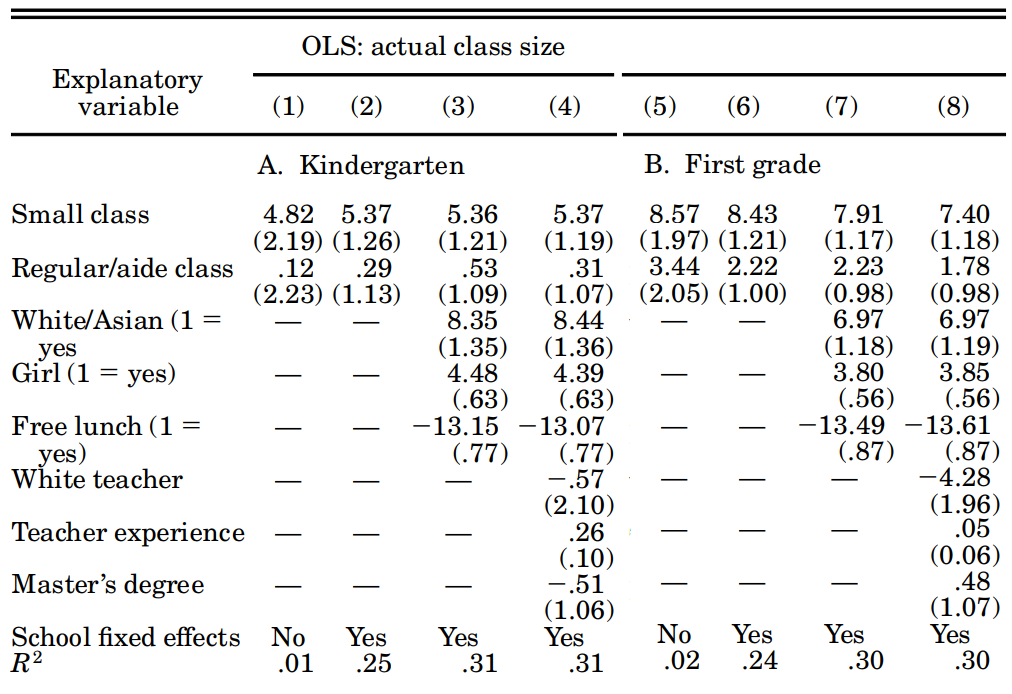
\includegraphics[width=0.7\textwidth]{./Figures/krueger.png}
\end{center}

\end{frame}

%\begin{frame}{Some difficulties for running field experiments}
%Attrition
%A Common Problem in Randomized Experiments
%If attrition is random and a¤ects the treatment and control groups in
%the same way the estimates would remain unbiased.
%Here the attrition is likely to be non-random: especially good students
%from large classes may have enrolled in private schools creating a
%selection bias problem.
%Krueger addresses this concern by imputing test scores (from their
%earlier test scores) for all children who leave the sample and then
%reestimates the model including students with imputed test scores.
%Waldinger
%\end{frame}

\begin{frame}{Some difficulties for running field experiments}
\textbf{1- Randomization-out} or \textbf{Randomization Bias}:\medskip

Some people may not participate in the study. If nonparticipants are systematically different from participant the findings are not applicable to them.\bigskip

This problem occurs when the treatment effect is heterogeneous. %The experimental sample may be different from the population of interest because of randomization. 
People selecting to take part in the randomized trial
may have different returns compared to the population average.\bigskip

\textbf{2- Attrition bias}:\medskip

Attrition rates (i.e. leaving the sample between the baseline and the follow-up surveys) may be different in treatment and control groups.

The estimated treatment effect may therefore be biased.
\end{frame}

\begin{frame}{Some difficulties for running field experiments}
\textbf{3- Noncompliance} or \textbf{Substitution Bias}:\medskip

Control group members may seek or get substitutes for treatment.\medskip

This would bias estimated treatment effects downwards.\medskip

Can also occur if the experiment frees up resources that can now be concentrated on the control group.\bigskip

\textbf{4- Supply Side Changes}
If programmes are scaled up the supply side implementing the
treatment may be different and not motivated as the trial phase.
\end{frame}

\begin{frame}{Some difficulties for running field experiments}
\textbf{5-Hawthorne effect}: \medskip

Abnormal behaviour of treated subjects knowing that they are in a fishbowl
\begin{itemize}
\item For solving this one should run experiment with ``blinded'' subjects
\item This in done in medical science with placebo test but not always possible in social science
\item A placebo job training with junk knowledge??
\end{itemize}
If people from the control group behave differently these effects are sometimes called "John Henry" effects.\bigskip

\textbf{6- Moral issues}: if a treatment is perceived to be harmful (e.g. smoking) randomization is morally wrong.
\end{frame}

\begin{frame}{Example: Krueger (1999)}
\textbf{Attrition problem}\medskip

In STAR experiment the attrition is likely to be non-random: especially good students from large classes may have enrolled in private schools creating a selection bias problem.\medskip

Krueger addresses this concern by imputing test scores (from their earlier test scores) for all children who leave the sample and then reestimates the model including students with imputed test scores.
\end{frame}

\begin{frame}{Example: Krueger (1999)}
\textbf{Noncompliance problem}\medskip

Subjects moved between treatment and control groups.\medskip

A common solution to this problem is to use initial assignment (here initial assignment to small or regular classes) as an instrument for actual assignment.\medskip

Krueger reports reduced form results where he uses initial assignment and not current status as explanatory variable.\medskip

In Kindergarten OLS and reduced form are the same because students remained in their initial class for at least one year.\medskip

From grade 1 onwards OLS (column 1-4) and reduced form (columns
5-8) are different.
\end{frame}


%\begin{frame}{References:}
%\bibliographystyle{apalike}
%\small
%\bibliography{references}
%\end{frame}

\end{document}
